% 2D polar-vs-Cartesian coordinates sketch: an ellipse (red), a horizontal
% reference axis and radius vector r at angle \angtheta to a point on the
% ellipse (blue), labelled both as (x,y) and (r,\angtheta).
%
% Compile standalone with:  pdflatex 极坐标_tikz.tex
\documentclass[tikz,border=6pt]{standalone}
\usepackage{amsmath}
\usetikzlibrary{arrows.meta, calc}

\begin{document}
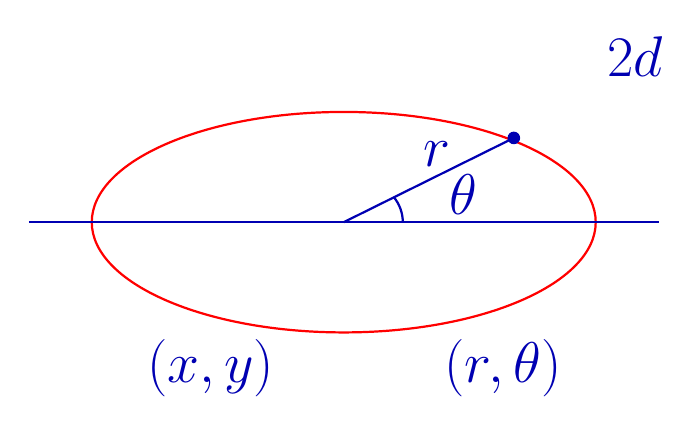
\begin{tikzpicture}[>=Stealth, thick, every node/.style={font=\fontsize{20}{24}\selectfont}]

  % ---- geometry -----------------------------------------------------
  \def\ea{3.2}   % ellipse semi-axis (horizontal)
  \def\eb{1.4}   % ellipse semi-axis (vertical)
  \def\angtheta{40} % angle of r, in degrees

  % ---- the ellipse (red) ----------------------------------------------
  \draw[red] (0,0) ellipse [x radius=\ea, y radius=\eb];

  % ---- horizontal reference line (blue) --------------------------------
  \draw[blue!70!black] (-4.0,0) -- (4.0,0);

  % ---- radius vector r at angle theta, ending on the ellipse ------------
  \coordinate (P) at (2.16,1.07);
  \draw[blue!70!black] (0,0) -- (P);
  \fill[blue!70!black] (P) circle (0.08cm);
  \node[blue!70!black] at ($(0,0)!0.55!(P)+(0,0.28)$) {$r$};

  % ---- angle arc + theta label ------------------------------------------
  \draw[blue!70!black] (0.75,0) arc[start angle=0, end angle=\angtheta, radius=0.5];
  \node[blue!70!black] at (1.52,0.35) {$\theta$};

  % ---- labels -------------------------------------------------------
  \node[blue!70!black] at (-1.69,-1.85) {$(x,y)$};
  \node[blue!70!black] at (2.02,-1.85) {$(r,\theta)$};
  \node[blue!70!black] at (3.7,2.1) {$2d$};

\end{tikzpicture}
\end{document}
